\scanpage{150}\mspage{5}
following two axioms

a) $d$ commutes with the operations of $L_0$, when one lets it act on $L_1$ by $\unsure{\Theta|\theta}\deleted{\unsure{s|,}}$, on itself by inner automorphisms:
\[
d\bigl(\Theta(x_0)\mathbin{.}x_1\bigr)=\mathrm{int}(x_0)\,d(x_1)
\]
\[
\Theta(d.(x_1))=\mathrm{int}(x_1)\tag*{\makebox[0pt][r]{\makebox[\displaywidth][l]{b)}}}
\]
These properties imply that $\mathrm{Im}\,d$ is \unsure{normal} in $L_0$ (hence $\unsure{\mathrm{Coker}|\mathrm{CoKer}}\,d=\unsure{\pi|\Pi}_0$ is defined) and $\pi_1=\mathrm{Ker}\,d$ is central in $L_1$, finally that $L_0$ acts on $L_1$ leaving $\pi_1$ invariant, and that it acts via $\pi_0$. The principal \inserted{cohomological} invariant of the situation is obviously the \unsure{Postnikoff|Postnikuff}-Sinh invariant
\[
\alpha\in\unsure{.}\,H^3(\pi_0,\pi_1).
\]

I have encountered these animals -- without even looking for them -- in quite a few situations, which I am not going to review for you here (I have moreover just \unsure{come across} them again in connection with the classification of ``ordinary'' formal groups \unsure{over|\deleted{\illegible{1}}over} a perfect field, in terms of \uline{affine} alg\unsure{e|e}braic groups\unsure{,|;} of \uline{commutative} formal groups, linked by strict Gr-structures of this type%
% margin note written sideways; the guide ends beside the line beginning strictes, without an exact word anchor
% The guide below is reproduced in the original page orientation; the note text is read upright.
\margin{\illegible{4} this formalism on an arbitrary topos (not only in $(\mathrm{Ens})$)
\figure{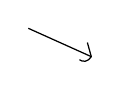
\begin{tikzpicture}[x=1cm,y=1cm]
\draw[line width=.45pt] (0,.36) -- (.80,0);
\draw[line width=.45pt] (.75,.18) -- (.80,0) .. controls (.76,-.07) and (.69,-.07) .. (.65,-.04);
\end{tikzpicture}}} -- to make explicit the yoga that ``the transcendental \unsure{character|character} \unsure{of the|of the}
% archive sheet number: 150
